\newpage
\chapter{Coordinate Transformations}

\localtableofcontents*

\newpage

\section{Constructing Transformation Matrix}

\subsection{Rotation Matrix}

From: \href{https://mathworld.wolfram.com/RotationMatrix.html}{wolfram}

\begin{enumerate}
    \item 2-D (in $\mathbb{R}^{2}$):

        Rotating an object to a new coordinate system:

        \begin{figure}[ht]
            \centering
            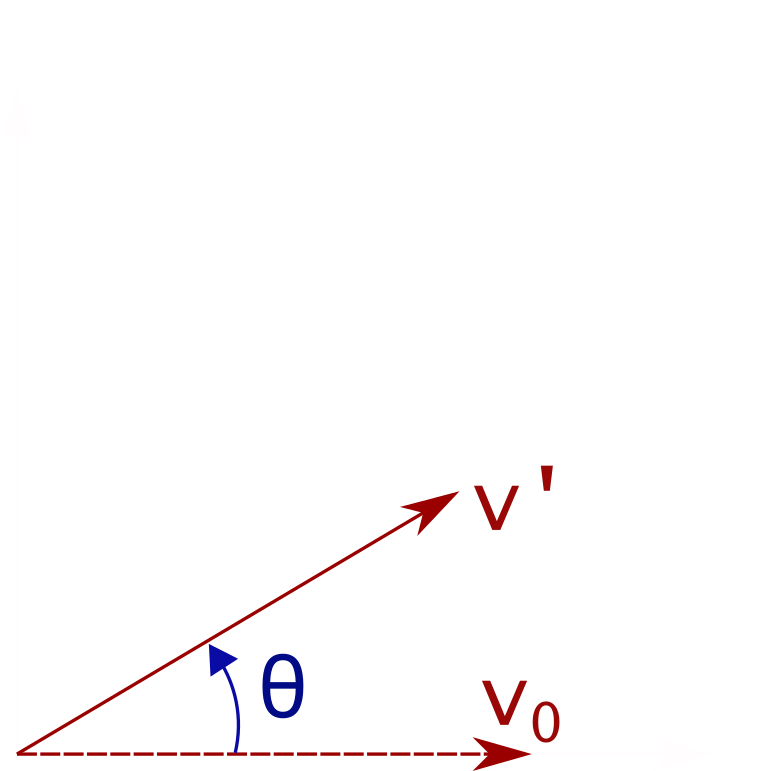
\includegraphics[width=0.35\textwidth]{img/RotationMatrix_1000}
            \caption{Rotating object}
            \label{fig:RotationMatrix_1000-png}
        \end{figure}

        In $\mathbb{R}^{2}$, consider the matrix that rotates a given
        vector $\mathbf{v}_{0}$ by a counterclockwise angle $\theta$ in
        a fixed coordinate system. Then

        \begin{equation}
            \mathbf{T}_{\theta} = \begin{bmatrix}
                \cos \theta & -\sin \theta \\
                \sin \theta & \cos \theta
            \end{bmatrix}
        ,\end{equation}

        so

        \begin{equation}
            \mathbf{v}^{'} = \mathbf{T}_{\theta}\mathbf{v}_{0}
        .\end{equation}

        \begin{figure}[ht]
            \centering
            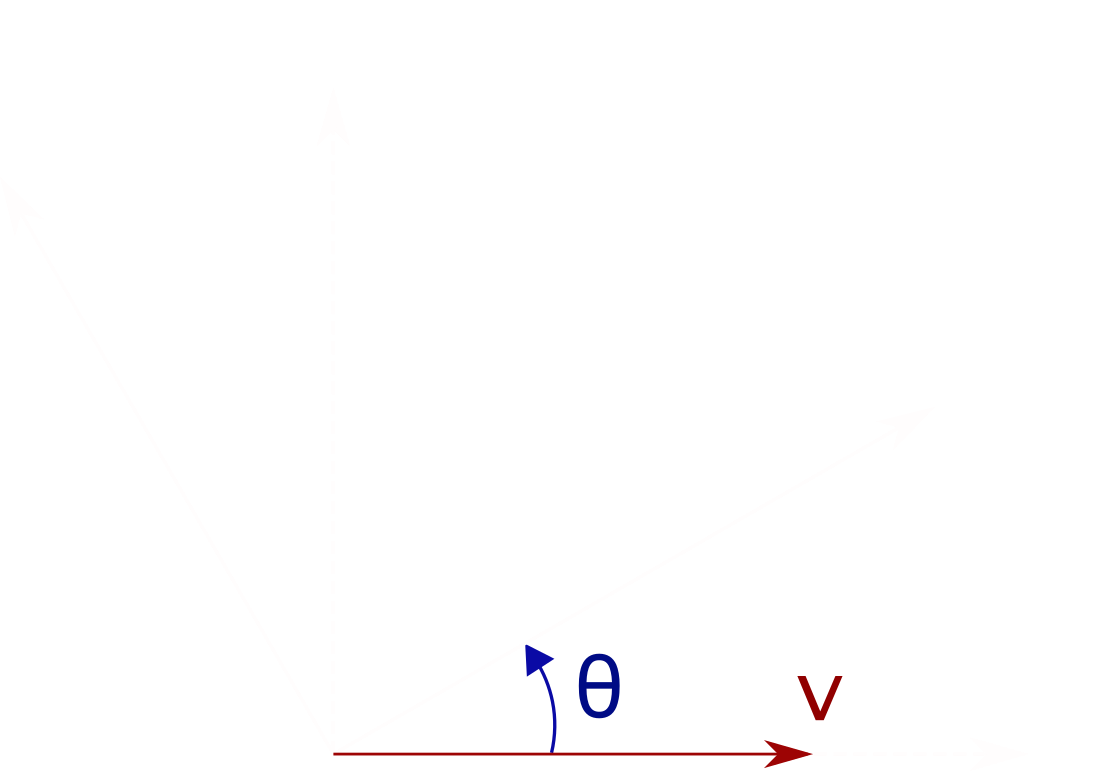
\includegraphics[width=0.5\textwidth]{img/RotationMatrixAxes_1000}
            \caption{Rotating Axes}
            \label{fig:RotationMatrixAxes_1000-png}
        \end{figure}

        On the other hand, consider the matrix that rotates the
        \textit{coordinate system} through a counterclockwise angle $\theta$.
        The coordinates of the fixed vector $\mathbf{v}$ in the rotated
        coordinate system are now given by a rotation matrix which is the
        \textit{transpose} of the fixed-axis matrix, as can be seen on the
        second figure, is equivalent to rotating the vector by
        a counterclockwise angle $-\theta$ relative to a fixed set of axes,
        giving:

        \begin{equation}
            \mathbf{T}_{\theta}^{'} = \begin{bmatrix}
                \cos \theta & \sin \theta \\
                -\sin \theta & \cos \theta
            \end{bmatrix}
        .\end{equation}

        This is the convention commonly used in textbooks.

    \item 3-D ($\mathbb{R}^{3}$):

        In $\mathbb{R}^{3}$, coordinate system rotations of the
        \textit{x-}, \textit{y-} and \textit{z-axis} in a counterclockwise
        direction when looking towards the origin give the matrices:

        \begin{equation}
            \mathbf{R}_{x}(\varphi) =
            \begin{bmatrix}
                1 & 0 & 0 \\
                0 & \cos \varphi & \sin \varphi \\
                0 & -\sin \varphi & \cos \varphi
            \end{bmatrix}
        .\end{equation}

        \begin{equation}
            \mathbf{R}_{y}(\theta) =
            \begin{bmatrix}
                \cos \theta & 0 & -\sin \theta \\
                0 & 1 & 0 \\
                \sin \theta & 0 & \cos \theta
            \end{bmatrix}
        .\end{equation}

        \begin{equation}
            \mathbf{R}_{z}(\psi) =
            \begin{bmatrix}
                \cos \psi & \sin \psi & 0 \\
                -\sin \psi & \cos \psi & 0 \\
                0 & 0 & 1
            \end{bmatrix}
        .\end{equation}

        Any \textbf{rotation} can be given as a composition of rotations
        about three axes (\textbf{Euler's rotation theorem}), and thus
        be represented by a $3 \times 3$ matrix operating on a vector.

        \begin{equation}
            \begin{bmatrix}
                x_{1}^{'} \\ x_{2}^{'} \\ x_{3}^{'}
            \end{bmatrix}
            =
            \begin{bmatrix}
                t_{11} & t_{12} & t_{13} \\
                t_{21} & t_{22} & t_{23} \\
                t_{31} & t_{32} & t_{33}
            \end{bmatrix}
            \begin{bmatrix}
                x_{1} \\ x_{2} \\ x_{3}
            \end{bmatrix}
        .\end{equation}

    \item \textbf{Euler's angles of XYZ rotation:}

        With the order of \textit{xyz} rotation the rotation matrix is
        composed as:

        \begin{equation}
            \scalebox{0.85}{
                $ \begin{array}{ll}
                    \mathbf{T}
                    &= \mathbf{R}_{z}(\psi)\mathbf{R}_{y}(\theta)\mathbf{R}_{x}(\varphi) \\
                    &=
                    \begin{bmatrix}
                        \cos \psi & \sin \psi & 0 \\
                        -\sin \psi & \cos \psi & 0 \\
                        0 & 0 & 1
                    \end{bmatrix}
                    \begin{bmatrix}
                        \cos \theta & 0 & -\sin \theta \\
                        0 & 1 & 0 \\
                        \sin \theta & 0 & \cos \theta
                    \end{bmatrix}
                    \begin{bmatrix}
                        1 & 0 & 0 \\
                        0 & \cos \varphi & \sin \varphi \\
                        0 & -\sin \varphi & \cos \varphi
                    \end{bmatrix} \\
                    &=
                    \begin{bmatrix}
                        \cos \theta \cos \psi
                        & \cos \psi \sin \theta \sin \varphi - \cos \varphi \sin \psi
                        & \cos \varphi \cos \psi \sin \theta + \sin \varphi \sin \psi \\
                        \cos \theta \sin \psi
                        & \cos \varphi \cos \psi + \sin \theta \sin \varphi \sin \psi
                        & \cos \varphi \sin \theta \sin \psi - \cos \psi \sin \varphi \\
                        -\sin \theta
                        & \cos \theta \sin \varphi
                        & \cos \theta \cos \varphi
                    \end{bmatrix}
                \end{array} $
            }
        \end{equation}

        Then the three \textit{Euler angles} for a \textit{xyz} rotation
        can be obtained:

        \begin{equation}
            \varphi = \atantwo(t_{32}, t_{33})
        ,\end{equation}

        \begin{equation}
            \theta = \atantwo \left(-t_{31}, \sqrt{ t_{32}^{2} + t_{33}^{2}} \right)
        ,\end{equation}

        \begin{equation}
            \psi = \atantwo(t_{21}, t_{11})
        ,\end{equation}

        where $\atantwo(y, x)$ definition is:

        \begin{equation}
            \atantwo(y, x) = \left\{
                \begin{array}{ll}
                    \arctan\left(\frac{y}{x}\right) & if \quad (x > 0),\\
                    \arctan\left(\frac{y}{x}\right) + \pi & if \quad (x < 0) \land (y \ge 0),\\
                    \arctan\left(\frac{y}{x}\right) - \pi & if \quad (x < 0) \land  (y < 0),\\
                    \frac{\pi}{2} & if \quad (x = 0) \land  (y > 0),\\
                    -\frac{\pi}{2} & if \quad (x = 0) \land  (y < 0),\\
                    undefined & if \quad (x = 0) \land (y = 0)
                \end{array}
            \right\}
        .\end{equation}

        \textbf{Note} the angle limitation for values returned while doing
        an Euler angle decomposition of a \textbf{rotation} matrix:

        \begin{equation}
            \begin{array}{l}
                \varphi \in (-\pi, \pi) \\
                \theta \in (-\frac{\pi}{2}, \frac{\pi}{2}) \\
                \psi \in (-\pi, \pi)
            \end{array}
        .\end{equation}

    \item Euler's angles of \textbf{ZYX} rotation:

        For a rotation defined in \textit{zyx} order the rotation matrix is:

        \begin{equation}
            \scalebox{0.85}{
                $ \begin{array}{ll}
                    \mathbf{T}
                    &= \mathbf{R}_{x}(\varphi)\mathbf{R}_{y}(\theta)\mathbf{R}_{z}(\psi) \\
                    &=
                    \begin{bmatrix}
                        1 & 0 & 0 \\
                        0 & \cos \varphi & \sin \varphi \\
                        0 & -\sin \varphi & \cos \varphi
                    \end{bmatrix}
                    \begin{bmatrix}
                        \cos \theta & 0 & -\sin \theta \\
                        0 & 1 & 0 \\
                        \sin \theta & 0 & \cos \theta
                    \end{bmatrix}
                    \begin{bmatrix}
                        \cos \psi & \sin \psi & 0 \\
                        -\sin \psi & \cos \psi & 0 \\
                        0 & 0 & 1
                    \end{bmatrix} \\
                    &=
                    \begin{bmatrix}
                        \cos \theta \cos \varphi
                        & - \cos \theta \sin \varphi
                        & \sin \varphi \\
                        \cos \psi \sin \varphi + \cos \varphi \sin \theta \sin \psi
                        & \cos \varphi \cos \psi - \sin \theta \sin \varphi \sin \psi
                        & -\cos \theta \sin \psi \\
                        \sin \varphi \sin \psi - \cos \varphi \cos \psi \sin \theta
                        & \cos \psi \sin \theta \sin \varphi + \cos \varphi \sin \psi
                        & \cos \theta \cos \psi
                    \end{bmatrix}
                \end{array} $
            }
        .\end{equation}

        \textbf{Note that the angles $\varphi$, $\theta$ and $\psi$ defined here are
        different from the \textit{XYZ} rotation defined above!} The rotation
        is performed by first rotating around \textit{z-axis} counterclockwise
        by an angle $\psi$, then around \textit{y-axis} counterclockwise
        by an angle $\theta$ and finaly around \textit{x-axis}, counterclockwise,
        by an angle $\varphi$.

        Then the \textit{Euler's angles} can be obtained as:

        \begin{equation}
            \left\{ \begin{array}{l}
                \varphi = \arctan \left( \frac{-t_{12}}{t_{11}} \right)\\
                \theta = \arcsin \left( t_{13} \right) \\
                \psi = \arctan \left( \frac{-t_{23}}{t_{33}} \right)
            \end{array} \right.
        .\end{equation}


    \item Alternate way of constructing \textbf{Rotation matrix} without specifying
        angles:

        The rotation matrix to a new coordinate system can be constructed from
        its axes, where the rotation matrix can be defined as:

        \begin{equation}
            \mathbf{T}_{R} = \begin{bmatrix}
                x_1 & x_2 & x_3 \\
                y_1 & y_2 & y_3 \\
                z_1 & z_2 & z_3 \\
            \end{bmatrix}
        ,\end{equation}

        where $\mathbf{x} = [x_1, x_2, x_3]^{T}$, $\mathbf{y} = [y_1, y_2, y_3]^{T}$
        and  $\mathbf{z} = [z_1, z_2, z_3]^{T}$ are unit vectors in the direction
        of \textit{x-}, \textit{y-} and \textit{z-axis} of the new coordinate
        system.


        \begin{bbox}[0.85]
            The \textbf{transformation matrix} can be defined by any two vectors
            $\mathbf{u}$ and $\mathbf{v}$, where $\mathbf{u}$ defines the direction
            of \textit{x-axis} and $\mathbf{v}$ defines the \textit{xy-plane}.
            To construct the \textbf{rotation matrix} use the following steps:

            \begin{enumerate}
                \item create x-axis of unit lenght

                    \begin{equation}
                        \mathbf{x} = \frac{\mathbf{u}}{||\mathbf{u}||}
                    .\end{equation}

                \item create z-axis of unit lenght

                    \begin{equation}
                        \mathbf{z}
                        = \frac{\mathbf{u} \times \mathbf{v}}{||\mathbf{u} \times \mathbf{v}||}
                    .\end{equation}

                \item create y-axis of unit lenght

                    \begin{equation}
                        \mathbf{y}
                        = \frac{\mathbf{z} \times \mathbf{x}}{||\mathbf{z} \times \mathbf{x}||}
                    .\end{equation}

                \item compose \textbf{rotation matrix}

                    \begin{equation}
                        \mathbf{T}_{R} = \begin{bmatrix}
                            \mathbf{x}^{T} \\
                            \mathbf{y}^{T} \\
                            \mathbf{z}^{T}
                        \end{bmatrix}
                    .\end{equation}
            \end{enumerate}

            The creation of the \textbf{rotation matrix} by any two other vectors is
            analogic, as \textbf{orthogonal} base must be constructed first, then
            the matrix is composed of its vectors.
        \end{bbox}

        \begin{bbox}[0.85]
            To test, whether the transformation matrix is correct, one can use
            the orthogonality criterion:

            \begin{equation}
                \mathbf{T}^{T} = \mathbf{T}^{-1}
            .\end{equation}

            \begin{equation}
                \mathbf{T}\mathbf{T}^{T} = \mathbf{T}^{T}\mathbf{T} = \mathbf{I}
            .\end{equation}

            or

            \begin{equation}
                \det(\mathbf{T}) = 1
            .\end{equation}
        \end{bbox}

\end{enumerate}


\section{Coordinate Transformation}

\begin{itemize}
    \item \textbf{Rotation:}

        Let $\mathbf{A}^{T} = [a_{x}, a_{y}, a_{z}]$ be the original coordinates,
        $\mathbf{B}^{T} = [b_{x}, b_{y}, b_{z}]$ be the transformed coordinates, and
        $\mathbf{T}$ a tranformation matrix in the form:

        \begin{equation}
            \mathbf{T} = \begin{bmatrix}
                x_1 & x_2 & x_3 \\
                y_1 & y_2 & y_3 \\
                z_1 & z_2 & z_3
            \end{bmatrix} = \begin{bmatrix}
                \mathbf{x} \\
                \mathbf{y} \\
                \mathbf{z}
            \end{bmatrix}
        ,\end{equation}

        where $\mathbf{x} = [x_1, x_2, x_3]$, $\mathbf{y} = [y_1, y_2, y_3]$ and
        $\mathbf{z} = [z_1, z_2, z_3]$ are the \textit{x-axis}, \textit{y-axis} and
        \textit{z-axis} \textbf{unit vectors}, respectively, of the new coordinate
        system defined in the original one, while sharing their origin.

        The following applies:

        \begin{equation}
            \mathbf{T} \times \mathbf{A} = \mathbf{B}
        ,\end{equation}

        and

        \begin{equation}
            \mathbf{T}^{T} \times \mathbf{B} = \mathbf{A}
        .\end{equation}

        \textbf{Note:} Perpendicular vector is  created using \textit{cross-product}.
\end{itemize}


\section{Tensor Transformation}

From:

\href{https://wp.optics.arizona.edu/optomech/wp-content/uploads/sites/53/2016/10/OPTI_222_W21.pdf}{source 1},
\href{https://www.continuummechanics.org/principalstressesandstrains.html}{source 2},
\href{https://www.ecourses.ou.edu/cgi-bin/eBook.cgi?doc=&topic=me&chap_sec=07.2&page=theory}{source 3}

Let real symmetric matrix  $\mathbf{A}$ be the original tensor,
real symmetric matrix $\mathbf{B}$ the transformed tensor, and
orthogonal matrix $\mathbf{T}$ a tranformation matrix in the form:

\begin{equation}
    \mathbf{A} = \begin{bmatrix}
        \sigma^{A}_{11} & \sigma^{A}_{12} & \sigma^{A}_{13} \\
        \sigma^{A}_{21} & \sigma^{A}_{22} & \sigma^{A}_{23} \\
        \sigma^{A}_{31} & \sigma^{A}_{32} & \sigma^{A}_{33}
    \end{bmatrix}
,\end{equation}

\begin{equation}
    \mathbf{B} = \begin{bmatrix}
        \sigma^{B}_{11} & \sigma^{B}_{12} & \sigma^{B}_{13} \\
        \sigma^{B}_{21} & \sigma^{B}_{22} & \sigma^{B}_{23} \\
        \sigma^{B}_{31} & \sigma^{B}_{32} & \sigma^{B}_{33}
    \end{bmatrix}
,\end{equation}

\begin{equation}
    \mathbf{T} = \begin{bmatrix}
        x_1 & x_2 & x_3 \\
        y_1 & y_2 & y_3 \\
        z_1 & z_2 & z_3
    \end{bmatrix} = \begin{bmatrix}
        \mathbf{x} \\
        \mathbf{y} \\
        \mathbf{z}
    \end{bmatrix}
,\end{equation}

where $\mathbf{x} = [x_1, x_2, x_3]$, $\mathbf{y} = [y_1, y_2, y_3]$ and
$\mathbf{z} = [z_1, z_2, z_3]$ are the \textit{x-axis}, \textit{y-axis} and
\textit{z-axis} \textbf{unit vectors}, respectively, of the new coordinate
system defined in the original one, while sharing their origin.

The transformation matrix $\mathbf{T}$ must satisfy
$\mathbf{T}\mathbf{T}^{T} = \mathbf{T}^{T}\mathbf{T} = \mathbf{I}$, where $\mathbf{I}$
is an identity matrix. This means that transformation matrix must be orthogonal,
therefore satisfying $\mathbf{T}^{T} = \mathbf{T}^{-1}$.

Then \textbf{tensor transformation} is performed as such:

\begin{equation}
    \mathbf{T} \times \mathbf{A} \times \mathbf{T}^{T} = \mathbf{B}
.\end{equation}

\begin{equation}
    \mathbf{T}^{T} \times \mathbf{B} \times \mathbf{T} = \mathbf{A}
.\end{equation}

\begin{itemize}
    \item \textbf{Principal values:}

        The principal values can be found as the \textbf{eigenvalues} of the tensor
        matrix.

        Characteristic equation of tensor $\mathbf{\Sigma}$:

        \begin{equation}
            \mathbf{\Sigma}\mathbf{V} = \mathbf{\Lambda} \mathbf{V}
        ,\end{equation}

        therefore:

        \begin{equation}
            (\mathbf{\Sigma} - \mathbf{\Lambda}\mathbf{I})\mathbf{V} = 0
        ,\end{equation}

        and:

        \begin{equation}
            det(\mathbf{\Sigma} - \mathbf{\Lambda}\mathbf{I}) = 0
        ,\end{equation}

        where $\mathbf{\Lambda}$ is a diagonal matrix of eigenvalues (principal values)
        and $\mathbf{V}$ is the eigenvector matrix.

        The characteristic cubic equation can be also written as:

        \begin{equation}
            \lambda^{3} - I_{1}\lambda^{2} + I_{2}\lambda - I_{3} = 0
        ,\end{equation}

        giving three roots equal to tensor eigenvalues.

        First compute \textbf{Invariants} $\mathbf{I}_{n}$:

        \begin{equation}
            \begin{array}{ll}
                I_{1} &= \sigma_{11} + \sigma_{22} + \sigma_{33} \\
                I_{2} &= \sigma_{11}\sigma_{22} + \sigma_{22}\sigma_{33}
                + \sigma_{33}\sigma_{11} - \sigma_{12}^{2} - \sigma_{13}^{2} - \sigma_{23}^{2} \\
                I_{3}
                &= \sigma_{11}\sigma_{22}\sigma_{33}
                - \sigma_{11}\sigma_{23}^{2}
                - \sigma_{22}\sigma_{13}^{2}
                - \sigma_{33}\sigma_{12}^{2}
                + 2 \sigma_{12}\sigma_{13}\sigma_{23}
            \end{array}
        .\end{equation}

        In matrix form:

        \begin{equation}
            \begin{array}{ll}
                I_{1} &= tr[\mathbf{\Sigma}] \\
                I_{2} &= \left| \begin{matrix}
                    \sigma_{11} & \sigma_{12} \\
                    \sigma_{12} & \sigma_{22}
                \end{matrix} \right| + \left| \begin{matrix}
                    \sigma_{11} & \sigma_{13} \\
                    \sigma_{13} & \sigma_{33}
                \end{matrix} \right| + \left| \begin{matrix}
                    \sigma_{22} & \sigma_{23} \\
                    \sigma_{23} & \sigma_{33}
                \end{matrix} \right| \\
                    I_{3} &= det(\mathbf{\Sigma})
            \end{array}
        .\end{equation}

        Then compute \textit{help values}:

        \begin{equation}
            Q = \frac{3 I_{2} - I_{1}^{2}}{9}
        ,\end{equation}

        \begin{equation}
            R = \frac{2 I_{1}^{3} - 9 I_{1} I_{2} + 27 I_{3}}{54} \\
        ,\end{equation}

        \begin{equation}
            \theta = cos^{-1} \left( \frac{ R }{ \sqrt{- Q^{3}}} \right)
        .\end{equation}

        Lastly to get \textbf{principal values}:

        \begin{equation}
            \overline{\sigma_{1}}
            = 2 \sqrt{-Q} \cos{\left(\frac{\theta}{3}\right)} + \frac{1}{3}I_{1}
        .\end{equation}

        \begin{equation}
            \overline{\sigma_{2}}
            = 2 \sqrt{-Q} \cos{\left(\frac{\theta + 2 \pi}{3}\right)} + \frac{1}{3}I_{1}
        .\end{equation}

        \begin{equation}
            \overline{\sigma_{3}}
            = 2 \sqrt{-Q} \cos{\left(\frac{\theta + 4 \pi}{3}\right)} + \frac{1}{3}I_{1}
        .\end{equation}

        The \textbf{principal values are not sorted}. The principal tensor is then:

        \begin{equation}
            \mathbf{\Sigma} = \begin{bmatrix}
                \sigma_{1} & 0 & 0 \\
                0 & \sigma_{2}  & 0 \\
                0 & 0 & \sigma_{3}
            \end{bmatrix}
        ,\end{equation}

        where $\overline{\sigma}_{1}$, $\overline{\sigma}_{2}$ and $\overline{\sigma}_{3}$
        $\implies$ $\sigma_1 > \sigma_2 > \sigma_3$.

        Afterwards the \textbf{principal axes} are obtained as:

        \begin{equation}
            \begin{array}{l}
                \mathbf{\Gamma}_{1} = \mathbf{\Sigma} - \sigma_{1}\mathbf{I} \\
                \mathbf{\Gamma}_{2} = \mathbf{\Sigma} - \sigma_{2}\mathbf{I} \\
                \mathbf{\Gamma}_{3} = \mathbf{\Sigma} - \sigma_{3}\mathbf{I}
            \end{array}
        ,\end{equation}

        where $\mathbf{\Gamma}$ is a coordinate system corresponding to the
        principal value \textit{i} and $\mathbf{I}$ is a $3 \times 3$
        identity matrix.

        The vectors corresponding to each \textbf{principal value} are obtained:

        \begin{equation}
            \mathbf{\Gamma}_{1}
            = \begin{bmatrix}
                \overline{x}_{11} & \overline{x}_{12} & \overline{x}_{13}\\
                \overline{y}_{11} & \overline{y}_{12} & \overline{y}_{13}\\
                \overline{z}_{11} & \overline{z}_{12} & \overline{z}_{13}
            \end{bmatrix}
            = \begin{bmatrix}
                \overline{\mathbf{x}}_{1}\\
                \overline{\mathbf{y}}_{1}\\
                \overline{\mathbf{z}}_{1}
            \end{bmatrix}
        ,\end{equation}
        \begin{equation}
            \mathbf{\Gamma}_{2}
            = \begin{bmatrix}
                \overline{x}_{21} & \overline{x}_{22} & \overline{x}_{23}\\
                \overline{y}_{21} & \overline{y}_{22} & \overline{y}_{23}\\
                \overline{z}_{21} & \overline{z}_{22} & \overline{z}_{23}
            \end{bmatrix}
            = \begin{bmatrix}
                \overline{\mathbf{x}}_{2}\\
                \overline{\mathbf{y}}_{2}\\
                \overline{\mathbf{z}}_{2}
            \end{bmatrix} \\
        ,\end{equation}
        \begin{equation}
            \mathbf{\Gamma}_{3}
            = \begin{bmatrix}
                \overline{x}_{31} & \overline{x}_{32} & \overline{x}_{33}\\
                \overline{y}_{31} & \overline{y}_{32} & \overline{y}_{33}\\
                \overline{z}_{31} & \overline{z}_{32} & \overline{z}_{33}
            \end{bmatrix}
            = \begin{bmatrix}
                \overline{\mathbf{x}}_{3}\\
                \overline{\mathbf{y}}_{3}\\
                \overline{\mathbf{z}}_{3}
            \end{bmatrix}
        ,\end{equation}

        where $\overline{\mathbf{x}}$, $\overline{\mathbf{y}}$ and $\overline{\mathbf{z}}$ are vectors of size 3.

        \begin{equation}
              \mathbf{x} = \frac{\overline{\mathbf{y}}_{1} \times \overline{\mathbf{z}}_{1}}
              {|\overline{\mathbf{y}}_{1} \times \overline{\mathbf{z}}_{1}|}\\
        ,\end{equation}
        \begin{equation}
              \mathbf{y} = \frac{\overline{\mathbf{z}}_{2} \times \overline{\mathbf{x}}_{2}}
              {|\overline{\mathbf{z}}_{2} \times \overline{\mathbf{x}}_{2}|}\\
        ,\end{equation}
        \begin{equation}
              \mathbf{z} = \frac{\overline{\mathbf{x}}_{3} \times \overline{\mathbf{y}}_{3}}
              {|\overline{\mathbf{x}}_{3} \times \overline{\mathbf{y}}_{3}|}
        .\end{equation}

        The principal axes are also the \textbf{eigenvectors} of tensor $\mathbf{\Sigma}$:

        \begin{equation}
            \mathbf{V} = \begin{bmatrix}
                \mathbf{x} & \mathbf{y} & \mathbf{z}
            \end{bmatrix} = \begin{bmatrix}
                x_1 & y_1 & z_1 \\
                x_2 & y_2 & z_2 \\
                x_3 & y_3 & z_3
            \end{bmatrix}
        .\end{equation}

    \item \textbf{Maximum Shear value:}


        Maximum \textbf{shear stress} occurs at an angle of 45 degrees to principal axes.
        If principal stresses are aligned such that $\sigma_1 > \sigma_2 > \sigma_3$
        and the stress tensor is:

        \begin{equation}
            \mathbf{\Sigma} = \begin{bmatrix}
                \sigma_1 & 0 & 0 \\
                0 & \sigma_2 & 0 \\
                0 & 0 & \sigma_3
            \end{bmatrix}
        ,\end{equation}

        then maximum shear stress $\tau_{max}$ can be obtained as follows:

        \begin{equation}
            \tau_{max} = \frac{\sigma_1 - \sigma_3}{2}
        \end{equation}

        and is at 45 degrees angle in the 1-3 plane of the principal axes to the
        principal coordinate system.

        More generally (in 2D):

        \begin{equation}
            \tau_{max} = \sqrt{\left(\frac{\sigma_{x} - \sigma_{y}}{2}\right)^{2}
            + \tau_{xy}^{2}}
        .\end{equation}

        \begin{bbox}[0.85]
            When the principal tensor is rotated by 45 degrees to obtain \textbf{maximum
            shear stress}, the axial stress components corresponding to this shear
            stress are equal.

            The value of maximal shear stress is obtained:

            \begin{equation}
                \tau_{max} = \frac{\sigma_{max} - \sigma_{min}}{2}
            .\end{equation}

            The value of axial stresses corresponding to maximal shear stress is
            the average of maximal and minimal axial stresses:

            \begin{equation}
                \sigma_{\tau_{max}} = \frac{\sigma_{max} + \sigma_{min}}{2}
            .\end{equation}

        \end{bbox}

    \item \textbf{Example:}

        Let a stress tensor in principal coordinate system be:

        \begin{equation}
             \mathbf{\Sigma} = \begin{bmatrix}
                 433 & 0 & 0 \\
                 0 & 125 & 0 \\
                 0 & 0 & 24
             \end{bmatrix}
        ,\end{equation}

        then $\sigma_1 = \sigma_{max} = 433 \text{ MPa}$ and
        $\sigma_3 = \sigma_{min} = 24 \text{ MPa}$.

        Transformation matrix for rotating by 45 degrees in 3-1 plane is:

        \begin{equation}
            \mathbf{T} = \begin{bmatrix}
                \frac{\sqrt{2}}{2} & 0 & -\frac{\sqrt{2}}{2} \\
                0 & 1 & 0 \\
                \frac{\sqrt{2}}{2} & 0 & \frac{\sqrt{2}}{2}
            \end{bmatrix}
        .\end{equation}

        Rotating tensor $\mathbf{\Sigma}$ by transformation matrix $\mathbf{T}$ we get:

        \begin{equation}
            \mathbf{\Sigma}_{\tau} = \mathbf{T}\mathbf{\Sigma}\mathbf{T}^{T}
            = \begin{bmatrix}
                228.5 & 0 & 204.5 \\
                0 & 125 & 0 \\
                204.5 & 0 & 228.5
            \end{bmatrix}
        ,\end{equation}

        where:

        \begin{equation}
            \begin{array}{l}
                \tau_{max} = \sigma_{13} = \sigma_{31} = 204.5 \\
                \sigma_{11} = \sigma_{33} = 228.5 \\
                \sigma_{22} = \sigma_2
            \end{array}
        .\end{equation}

        Check for correct values:

        \begin{equation}
            \tau_{max} = \frac{\sigma_1 - \sigma_3}{2} = \frac{433 - 24}{2}
            = \frac{409}{2} = 204.5 \text{ MPa} \implies \text{OK!}
        ,\end{equation}

        \begin{equation}
            \sigma_{11} = \sigma_{33} = \frac{\sigma_1 + \sigma_3}{2}
            = \frac{433 + 24}{2} = 228.5 \text{ MPa} \implies \text{OK!}
        .\end{equation}

        \textbf{$\sigma_2$ has not changed as it is colinear with the axis of rotation.}

        The relationship between principal normal streses and maximum shear stresses
        can be better understood by examining a plot of the stresses as a function
        of the rotation angle.

        Notice that there are multiple $\theta_{p}$ and $\theta_{\tau - max}$
        angles because of the periodical nature of the equations. However, they
        will give the same absolute values.

        At the principal stress angle, $\theta_{p}$, the shear stress will always be zero,
        as shown on the diagram. And the maximum shear stress will occur when the
        two principal normal stresses, $\sigma_1$ and $\sigma_2$, are equal.

        \begin{figure}[ht]
            \centering
            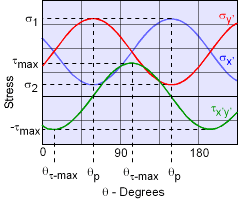
\includegraphics[width=0.8\textwidth]{img/stresses_as_function_of_angle}
            \caption{Stresses as a function of angle}
            \label{fig:stresses_as_function_of_angle-png}
        \end{figure}

        \begin{bbox}[0.85]
            When $\sigma_{x}$ or $\sigma_{y}$ are either max or min, the shear stress
            $\tau_{xy}$ is equal to 0. When shear stress $\tau_{xy}$ is max or min,
            the stresses $\sigma_{x}$ and $\sigma_{y}$ are equal to their average.
        \end{bbox}


\end{itemize}


\section{Moment of Inertia}

From: \href{https://en.wikipedia.org/wiki/Parallel_axis_theorem}{Parallel axis theorem}

\textit{Parallel axis theorem}, also known as \textit{Huygens-Steiner's theorem}
or just \textit{Steiner's theorem} can be used to determine the \textbf{moment of inertia}
or \textbf{second moment of area} of a rigid body about any axis, given the body's
moment of inertia about a parallel axis through the objects center of gravity
and the perpendicular distance between the axes.

Moment of Inertia = \textbf{tensor}.

\begin{itemize}
    \item \textbf{Steiner's share:}

        \begin{equation}
            \mathbf{I}_{ss} = m \times \begin{bmatrix}
                y^{2} + z^{2} & -xy & -xz \\
                -yz & x^{2} + z^{2} & -yz \\
                -zx & -zy & x^{2} + y^{2}
            \end{bmatrix}
        .\end{equation}

        \textbf{Identities for a skew-symmetric matrix}

        In order to compare formulations of the parallel axis theorem using
        skew-symmetric matrices and the tensor formulation, the following
        identities are useful.

        Let $[\mathbf{R}]$ be the skew-symmetric matrix associated with the
        position vector $\mathbf{R} = (x, y, z)$, then the product in
        the inertia matrix becomes:

        \begin{equation}
            -[\mathbf{R}][\mathbf{R}] = \begin{bmatrix}
                0 & -z & y \\
                z & 0 & -x \\
                -y & x & 0
            \end{bmatrix}^{2}
            = \begin{bmatrix}
                y^{2} + z^{2} & -xy & -xz \\
                -yz & x^{2} + z^{2} & -yz \\
                -zx & -zy & x^{2} + y^{2}
            \end{bmatrix}
        .\end{equation}

        This product can be computed using the matrix formed by the outer product
        $[\mathbf{R} \mathbf{R}^{T}]$ using the identity

        \begin{equation}
            \begin{array}{ll}
                 \\
                -[\mathbf{R}]^{2}
                &= |\mathbf{R}|^{2}|\mathbf{E}_{3}| - [\mathbf{R}\mathbf{R}^{T}] \\
                &= \begin{bmatrix}
                    x^{2} + y^{2} + z^{2} & 0 & 0 \\
                    0 & x^{2} + y^{2} + z^{2} & 0 \\
                    0 & 0 & 0
                \end{bmatrix} - \begin{bmatrix}
                    x^{2} & xy & xz \\
                    yx & y^{2} & yz \\
                    zx & zy & z^{2}
                \end{bmatrix}
            \end{array}
        ,\end{equation}

        where $[\mathbf{E}_{3}$ is the $n \times n$  identity matrix.

        Also notice, that

        \begin{equation}
            |\mathbf{R}|^{2} = \mathbf{R} \cdot \mathbf{R} = tr [\mathbf{R}\mathbf{R}^{T}]
        .\end{equation}

        where $tr$ denotes the sum of the diagonal elements of the outer product
        matrix, known as its \textit{trace}.

        To obtain matrix of moments of inertia by rotating about any random
        point $A$ while having the moment of inertia in the center of gravity of
        the object $\mathbf{I}_{COG}$ and the coordinate distance $d = [x, y, z]$
        between the point $A$ and \textbf{COG} we:

        \begin{enumerate}
            \item Compute the moment of inertia relative to point $A$

                 \begin{equation}
                    \mathbf{I}_{A} = \mathbf{I}_{COG} + m \times \mathbf{I}_{SS}^{A \to COG}
                .\end{equation}

            \item Transform the tensor $\mathbf{I}_{A}$ to new rotated coordinate
                system using transformation matrix $\mathbf{T}$:

                \begin{equation}
                    \mathbf{I}_{A}^{'} = \mathbf{T} \times \mathbf{I}_{A} \times \mathbf{T}^{T}
                .\end{equation}

            \item Subtract the \textbf{Steiner's share} relative to new \textbf{COG}

                \begin{equation}
                    \mathbf{I}_{COG}^{'} = \mathbf{I}_{A}^{'} - \mathbf{I}_{SS}^{A' \to COG'}
                .\end{equation}

        \end{enumerate}



\end{itemize}

